%%%%%%%%%%
% Basics %
%%%%%%%%%%

\chapter{Grundlagen}
\label{chapter:basics}

Dieses Kapitel beschäftigt sich mit den Grundlagen für die Problematik der Layout-Berechnung in Diagrammen. Zunächst werden in Abschnitt \ref{sec:disambiguation} die wichtigsten Begriffe eingeführt und erläutert. Anschließend werden in Abschnitt \ref{sec:aesthetics-criteria} die ästhetischen Prinzipien für das Layout von allgemeinen Graphen und Klassendiagrammen der Notationssprache UML\footnote{Unified Modeling Language (\url{http://www.uml.org})} zusammengefasst.

\section{Begriffsklärung}
\label{sec:disambiguation}

\subsection{Graphbasierte Diagramme}
\label{subsec:graph-based-diagrams}

Viele Diagramme, die sich mit einer visuellen Sprache beschreiben lassen, basieren auf der Struktur von Graphen, d.h. sie werden durch Knoten (engl. Node) und Kanten (engl. Edge bzw. Link) gebildet \cite{Eichelberger05Aesthetics}. Die grafische Repräsentation der graphbasierten Diagramme (manchmal in der Literatur auch Node-Link-Diagramme genannt) besteht aus der Zusammensetzung von Textelementen und geometrischen Objekten wie Rechtecke, Ellipsen und Linien \cite{Wybrow08Using}. Die Struktur von Graphen kann um die Möglichkeit der Verschachtelung von Knoten und deren Verbindungen durch Kanten erweitert werden \cite{Siebenhaller03Automatisches, Wybrow08Using}. Trotz des häufigen Einsatzes dieser Erweiterung in vielen Diagrammtypen wird sie für die Zwecke dieser Bachelor-Arbeit außer Acht gelassen.

Zu den graphbasierten Diagrammen gehört eine große Anzahl an Softwarediagrammen, wie z.B. Klassendiagramme\footnote{Obwohl der UML-Standard eine Verschachtelung der Klassen in Pakete zulässt, sind an dieser Stelle einfachere Varianten der Klassendiagramme gemeint, wie z.B. die konzeptuellen Klassendiagramme nach \cite{Ambler04UML-2-Class}.}, Objektdiagramme bzw. Use-Case-Diagramme der Notationssprache UML, Netzwerkdiagramme oder Flowcharts.

\subsection{Layout}
\label{subsec:layout}

Durch die Spezifikationen der konkreten Diagrammtypen wird in der Regel ausschließlich die Struktur und die grafische Repräsentation festgelegt. Dagegen wird die Bestimmung der konkreten Eigenschaften der geometrischen Objekte wie z.B. ihre Anordnung nicht spezifiziert. Diese kann sich nach Konventionen, den Präferenzen der Nutzer bzw. nach ästhetischen Prinzipien richten \cite{Maier12A-Pattern-based, Wybrow08Using}. Durch eine Anpassung dieser Eigenschaften kann zum einen die Lesbarkeit des Diagramms verbessert werden und zum anderen können bestimmte Eigenschaften des Diagramms hervorgehoben werden \cite{Maier12A-Pattern-based}. Weiterhin kann durch das Layout eine sekundäre Notation geschaffen werden, die dem Diagramm eine zusätzliche Bedeutung gibt \cite{SeyboldGlinz03An-Effective}. In den meisten Diagramm-Editoren ist die Erstellung des Layouts dem Nutzer überlassen, sie können aber auch durch einen automatischen Algorithmus berechnet werden \cite{Maier12A-Pattern-based}. Die einzelnen Ansätze für das Layout von Diagrammen werden im Kapitel \ref{chapter:existing-approaches} vorgestellt.

Das Layout eines Diagramms wird als eine Zuordnung von Layout-Eigenschaften zu den Objekten des Diagramms definiert. Zu den bedeutsamen Layout-Eigenschaften der graphbasierten Diagramme (siehe Abschnitt \ref{subsec:graph-based-diagrams}) gehören vor allem die Positionen und Größen der Knoten und Routen der Kanten.

\subsection{Mentales Modell}
\label{subsec:mental-map}

Während der Arbeit mit einem Diagramm wird durch den Nutzer ein mentales Modell (engl. mental map) entwickelt, was sich durch seine Wahrnehmung der Struktur und der Bedeutung auszeichnet \cite{Branke01Dynamic, GladischSchumann14Semi-Automatic}.

Wenn das Inhalt bzw. das Layout des Diagramms geändert werden, muss sich der Nutzer an diese Änderung anpassen. Insbesondere in dem Fall einer automatische Änderung ist es sehr wichtig, diese für den Nutzer möglichst nachvollziehbar durchzuführen, so dass das mentale Modell erhalten bleibt \cite{Branke01Dynamic, Maier12A-Pattern-based}.

\section{Ästhetische Prinzipien}
\label{sec:aesthetics-criteria}

Die Qualität des Layouts von graphbasierten Diagrammen wird anhand von ästhetischen Prinzipien bestimmt \cite{Maier12A-Pattern-based}. Sie beschreiben die Grundsätze für die grafische Darstellung der Elemente im Diagramm und deren Einhaltung führt zu übersichtlichen und verständlichen Zeichnungen \cite{Siebenhaller03Automatisches}. Eine besonders wichtige Rolle spielen sie in automatischen Layout-Algorithmen, die im statischen Kontext eingesetzt werden \cite{Maier12A-Pattern-based}.

Die ästhetischen Prinzipien werden zahlreich in der Literatur z.B. in \cite{Siebenhaller03Automatisches}, \cite{EichelbergerSchmid09Guidelines}, \cite{Ambler05The-Elements}, \cite{Eichelberger05Aesthetics} und \cite{ShieberKosak93Automating} beschrieben und nach verschiedenen Faktoren kategorisiert. Für die Zwecke dieser Arbeit wurde die Unterteilung der ästhetischen Prinzipien für allgemeine Graphen und für Klassendiagramme ähnlich wie in \cite{Siebenhaller03Automatisches} gewählt. Eine Auflistung und eine kurze Zusammenfassung der bedeutsamsten Vertreter beiden Gruppen folgt in den folgenden Abschnitten.

\subsection{Ästhetische Prinzipien für Graphen}
\label{subsec:aesthetics-criteria-graphs}

Wie bereits in Abschnitt \ref{subsec:graph-based-diagrams} erläutert wurde, bauen die graphbasierten Diagramme auf der Struktur der Graphen auf. Für diese Struktur lassen sich ästhetische Prinzipien aufstellen, obwohl die Graphen an sich keine semantische Information besitzen \cite{Siebenhaller03Automatisches}. Sie können in der folgenden Liste nachgelesen werden:

\begin{enumerate}[label={A.\arabic*}]
    \item \textbf{Einhaltung der Abstände von Elementen} Die Elemente im Diagramm sollten nicht zu nahe aneinander liegen. Insbesondere sollten sich die Knoten nicht überlappen und die Kanten sollten keine Knoten schneiden. Die Abstände und Längen der Kanten sollten optimal gewählt werden, so dass das Diagramm übersichtlich bleibt \cite{Siebenhaller03Automatisches, Ambler05The-Elements}.
    \item \textbf{Reduktion der Anzahl der Kantenkreuzungen} Da die allgemeinen Graphen nicht zwingend planar sind, lassen sich Kantenkreuzungen nicht vermeiden. Der Übersichtlichkeit halber sollte versucht werden, die Anzahl der Kantenkreuzungen zu minimieren \cite{Siebenhaller03Automatisches, EichelbergerSchmid09Guidelines}.
    \item \textbf{Reduktion der Anzahl der Kantenknicke} Die Kanten können durch direkte Linien, Kurven oder eine Zusammensetzung von Liniensegmenten repräsentiert werden. Durch die Aufteilung der Kante in Segmente entsteht an jedem Verbindungspunkt von zwei Liniensegmenten ein Knick. Da der Verlauf der Kanten mit vielen Knicken schwer zu folgen ist, sollte ihre Anzahl minimiert werden \cite{Siebenhaller03Automatisches}.
    \item \textbf{Orthogonalität der Kanten} Durch die Zusammensetzung der Kanten aus ausschließlich horizontalen und vertikalen Segmenten wird trotz der Enthaltung von Knicken die Übersichtlichkeit gefördert \cite{Siebenhaller03Automatisches}. Somit macht der Einsatz von orthogonalen Kanten durchaus Sinn. Insbesondere vermeidet dieses Prinzip unzulässige Winkel an den Kantenknicken \cite{Siebenhaller03Automatisches} oder sogar Krümmungen der Kanten \cite{Ambler05The-Elements}.
    \item \textbf{Optimale Ausnutzung der Zeichenfläche} Um die Diagramme übersichtlicher zu gestalten, sollten die Knoten im Diagramm ausgewogen verteilt und die Gesamtfläche minimiert werden \cite{EichelbergerSchmid09Guidelines, Siebenhaller03Automatisches}.
    \item \textbf{Symmetrie} Durch die symmetrische Anordnung von Elementen wird eine schnellere Erfassung einer Teilstruktur des Diagramms ermöglicht \cite{Eichelberger05Aesthetics, Ambler05The-Elements}. Obwohl dieses Prinzip oft mit anderen Prinzipien kollidiert, sollte es angestrebt werden \cite{Siebenhaller03Automatisches}.
\end{enumerate}

\subsection{Ästhetische Prinzipien für Klassendiagramme}
\label{subsec:aesthetics-criteria-class-diagrams}

Die Klassendiagramme gehören zu häufig eingesetzten Diagrammtypen der Notationssprache UML \cite{Fowler03UML-Distilled:}. Sie werden für die Beschreibung der statischen Struktur eines objekt-orientierten Systems verwendet und visualisieren die Klassen und ihre Beziehungen \cite{Siebenhaller03Automatisches, Ambler05The-Elements}. Sie können für verschiedene Zwecke eingesetzt werden, u.a. für die Untersuchung der Konzepte für die Umsetzung von Anforderungen oder für den detaillierten Entwurf eines Systems \cite{Ambler04UML-2-Class, Ambler05The-Elements}. Aufgrund der Vielseitigkeit dieses Diagrammtyps wurden die Klassendiagramme zum Schwerpunkt dieser Arbeit gewählt.

Die Problematik des Layouts von Klassendiagrammen wurde in vielen Arbeiten untersucht, z.B. in \cite{Siebenhaller03Automatisches}, \cite{Eichelberger05Aesthetics} oder \cite{Eiglsperger04Automatic}. Die in diesen Arbeiten vorgestellten Layout-Algorithmen berücksichtigen ästhetische Prinzipien, die auf den semantischen Eigenschaften der Klassendiagramme basieren. Eine Auswahl der bedeutsamen Prinzipien wird im Folgenden aufgelistet:

\begin{enumerate}[label={A.\arabic*}, resume]
    \item \textbf{Richtung von Kanten} Die Kanten in Klassendiagrammen teilen sich in hierarchische und nicht-hierarchische unter \cite{Eichelberger05Aesthetics}, was von der Art der Relation abgeleitet wird, die sie repräsentieren. Die hierarchischen Kanten (wie z.B. Vererbung) sollen vertikal verlaufen, während die nicht-hierarchischen Kanten (wie z.B. Assoziation) horizontal angeordnet werden sollen \cite{EichelbergerSchmid09Guidelines, Ambler05The-Elements}. Insbesondere wichtig ist dieses Prinzip für die Vererbungshierarchien, in den die Unterklassen unter den Oberklassen abgebildet werden und somit die Kanten in einer Richtung verlaufen.
    \item \textbf{Darstellung von Hierarchien} Durch die hierarchischen Knoten gebildete Hierarchien bilden den Gegenstand für weitere ästhetische Prinzipien. Zum einen sollen die Geschwisterknoten auf der gleichen Ebene platziert werden \cite{Siebenhaller03Automatisches}. Zum anderen sollen die Väterknoten im Bezug zu den Kinderknoten möglichst zentriert ausgerichtet werden \cite{EichelbergerSchmid09Guidelines, Siebenhaller03Automatisches}. Dies erweitert das Prinzip der Symmetrie \cite{EichelbergerSchmid09Guidelines} und wird insbesondere bei Baumstrukturen eingesetzt \cite{Siebenhaller03Automatisches}.
    \item \textbf{Darstellung der Vererbungsrelationen} Die Vererbungsrelation kann auf zwei Arten dargestellt werden. Entweder werden wie in Abbildung \ref{fig:inheritance-representations-a} einzelne Linien für die jeweiligen Relationen verwendet oder es wird in einer \enquote{Gabelform} wie in Abbildung \ref{fig:inheritance-representations-b} dargestellt \cite{Siebenhaller03Automatisches}. Obwohl nach dem Standard beide Optionen zulässig sind, wird die zuletzt genannte Option als übersichtlicher eingeschätzt, obwohl sie zusätzliche Kantenknicke einführt \cite{EichelbergerSchmid09Guidelines, Siebenhaller03Automatisches}.

\begin{figure}[hbt]
    \newcommand{\subfigurewidth}{0.4\textwidth}
    \newcommand{\graphicswidth}{0.95\linewidth}
    \centering
    \begin{subfigure}{\subfigurewidth}
        \centering
        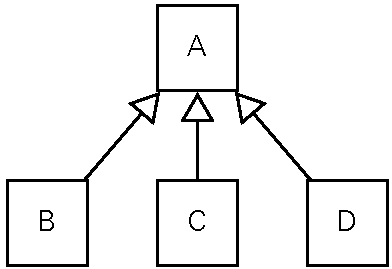
\includegraphics[width=\graphicswidth]{resources/inheritance-representations-a}
        \caption{}
        \label{fig:inheritance-representations-a}
    \end{subfigure}
    \begin{subfigure}{\subfigurewidth}
        \centering
        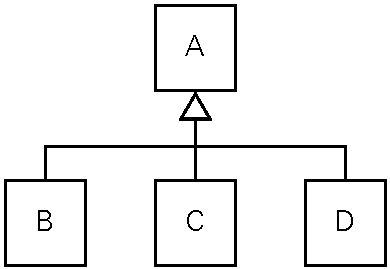
\includegraphics[width=\graphicswidth]{resources/inheritance-representations-b}
        \caption{}
        \label{fig:inheritance-representations-b}
    \end{subfigure}
    \caption{Möglichkeiten der Darstellung von Vererbungsrelationen in Klassendiagrammen}
    \label{fig:inheritance-representations}
\end{figure}

    \item \textbf{Platzierung von verwandten Elementen} Verwandte Elemente wie z.B. Pakete, durch Relationen verbundene Elemente, Vererbungshierarchien oder Design-Patterns sollen gruppiert und in der Nähe platziert werden \cite{Eichelberger05Aesthetics, Siebenhaller03Automatisches}. Weiterhin sollen die einzelnen Gruppen und insbesondere die Hierarchien im Diagramm verteilt werden \cite{Eiglsperger04Automatic}.
    \item \textbf{Platzierung von nicht verbundenen Elementen} Die Elemente, die über keine Verbindung zu anderen Elementen verfügen, sollen an der Seite der Zeichnung positioniert werden \cite{EichelbergerSchmid09Guidelines}.
\end{enumerate}
